\documentclass[../sparc.tex]{subfiles}
\graphicspath{{\subfix{../images/}}}
\begin{document}

%%%%%%%%%%%%%%%%%%%%%%%%%%%%%%%%%%%%%%%%%%%%%%%%%%%%%%%%%%%%%%%%%%%%%%%%%%%%%%%%
\section{Сборка электрической цепи}

Сложно говорить о современной цифровой технике без упоминания
\emph{микроконтроллера} -- ``мозга'' множества систем, с которыми мы
взаимодействуем каждый день.

Микроконтроллер -- это простой и обычно относительно дешёвый встраиваемый
компьютер, обычно решающий одну задачу.  Микроконтроллеры управляют современными
бытовыми приборами, игрушками, электронными музыкальными инструментами,
производственными роботами; на основе них работают 3D-принтеры и другие станки с
числовым программным управлением.

Мы будем работать с платформой Arduino, которая широко доступна и предоставляет
удобный интерфейс для её использования и программирования.

Внешний вид Arduino может различаться, в зависимости от модели; на
рис. \ref{fig:arduino-uno-r3} представлен один из популярных вариантов Arduino,
называемый ``Arduino UNO''.

\begin{figure}[ht]
  \centering
  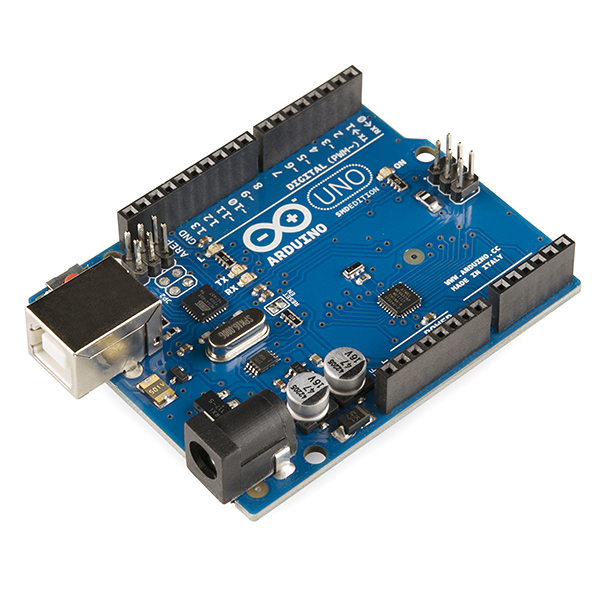
\includegraphics[width=12cm]{Arduino_Uno_-_R3}
  \caption{Микроконтроллерная платформа Arduino UNO R3.}
  \label{fig:arduino-uno-r3}
\end{figure}

Более подробно про использование платформы Arduino и её программирование речь
пойдёт в главе \ref{chapter:dialogues-with-computer}.  А пока что мы будем
использовать Arduino в качестве источника напряжения, вместо баратейки, которую
мы указывали до этого в схемах.

Как можно видеть на рисунке \ref{fig:arduino-uno-r3}, платформа имеет
специальные разъёмы, называемые \emph{портами}, для подключения компонентов и
проводов.  Есть порты, которые пронумерованы 0, 1, 2 и т.д. -- это
\emph{цифровые порты}.  Есть также порты, пронумерованные ``A0'', ``A1'', ``A2''
и т.д. -- это \emph{аналоговые порты}.  Цифровые и аналоговые порты мы пока
трогать не будем, так как для работы с ними требуется уже писать программу под
микроконтроллер; о написании программ мы поговорим позже.

Сейчас стоит обратить внимание на порты, обозначенные ``GND'' и ``5V''.  ``GND''
означает ``Ground'', или ``Земля'' -- это порт, на котором напряжение всегда
имеет значение ноль.  ``5V'' соответственно имеет всегда значение 5 Вольт.

Попробуем собрать электрическую цепь с резистором и светодиодом, приведённую на
рис. \ref{fig:electronics-arduino-circuit-00}.

\begin{figure}[ht]
  \centering
  \begin{circuitikz}
    \draw (3.5, 0) node[
      dipchip,
      num pins=2,
      external pins width=0.0,
      no topmark,
      hide numbers,
      xscale = 2.5,
      yscale = 2.5](C1){Arduino};
    \node [above left, font=\small] at (C1.bpin 1) {5V};
    \node [above right, font=\small] at (C1.bpin 2) {GND};
    \draw
    (C1.bpin 1) to[short]
    (0, 0) to[short]
    (0, 4) to[resistor, l=$R_1$] (3, 4)
    (3, 4) to[full led, l=Светодиод] (7, 4)
    (7, 4) to[short]
    (7, 0) to[short]
    (C1.bpin 2);
  \end{circuitikz}
  \caption{Схема подключения светодиода к Arduino.}
  \label{fig:electronics-arduino-circuit-00}
\end{figure}

Сборка схемы будет осуществляться на \emph{макетной плате} (англ.
\emph{breadboard} -- буквально ``хлебная доска''.)  Внешний вид макетной платы
показан на рис. \ref{fig:breadboard}.  На левой части рисунка показана лицевая
сторона макетной платы, куда вставляются детали при сборке схемы.  С правой
стороны рисунка показана обратная сторона макетной платы.  У новых макетных плат
обратная сторона обычно заклеена клейким слоем, поверх которого приклеет ещё
один защитный слой бумаги -- таким образом, макетную плату можно при
необходимости приклеить к чему-либо.  У макетной платы, показанной на
рис. \ref{fig:breadboard}, данный клейкий слой удалён для наглядности; без
особой на то необходимости лучше этот слой не убирать, так как он обеспечивает
изоляцию металлических контактов.

\begin{figure}[ht]
  \centering
  \caption{Макетная плата.}
  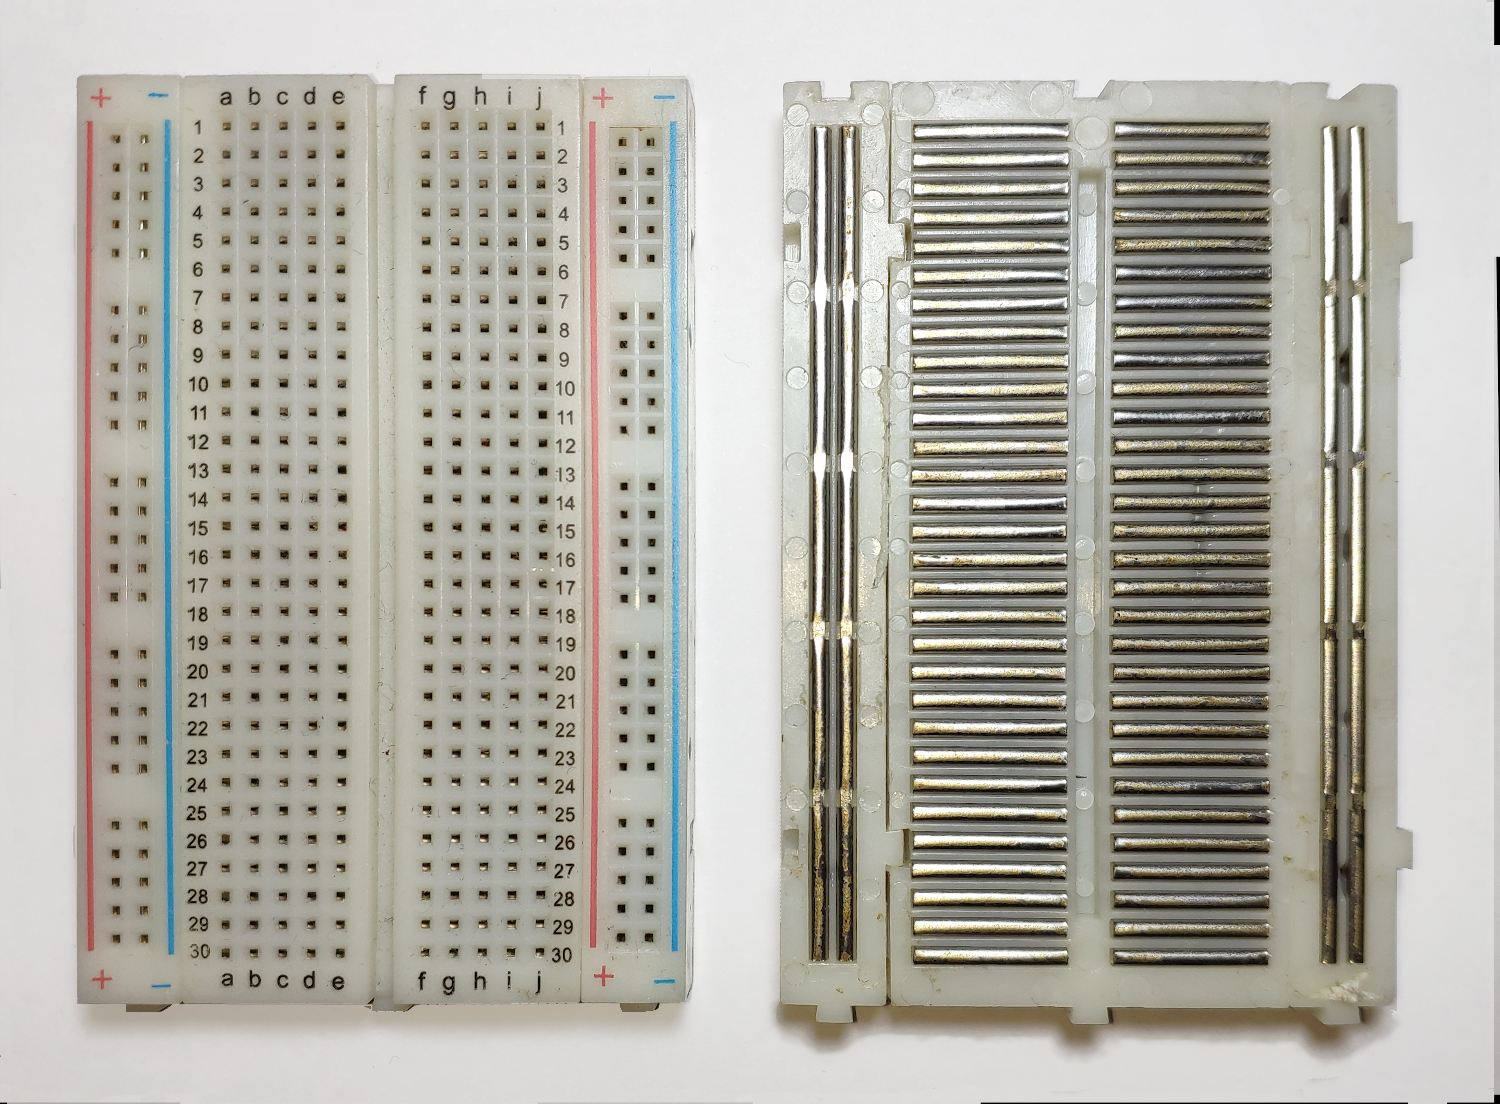
\includegraphics[width=12cm]{Breadboard}
  \label{fig:breadboard}
\end{figure}

Как можно видеть, макетная плата представляет собой просто сформованный кусок
пластика с вставленными в него металлическими контактами, обеспечивающими
соединение компонентов схемы, собираемой на ней.

Вдоль макетки, с каждой из сторон, располагаются две пары длинных линий,
помеченных на лицевой стороне макетной платы, как ``+'' и ``-'' -- эти линии
предназначены для организации общих линий питания и земли.

На макетной плате эта схема будет выглядеть следующим образом (см. рис.
\ref{fig:breadboard-simple-arduino-circuit}.)

\begin{figure}[ht]
  \centering
  \caption{Пример электрической цепи со светодиода и резистором, использующей
    Arduino UNO в качестве источника напряжения.}
  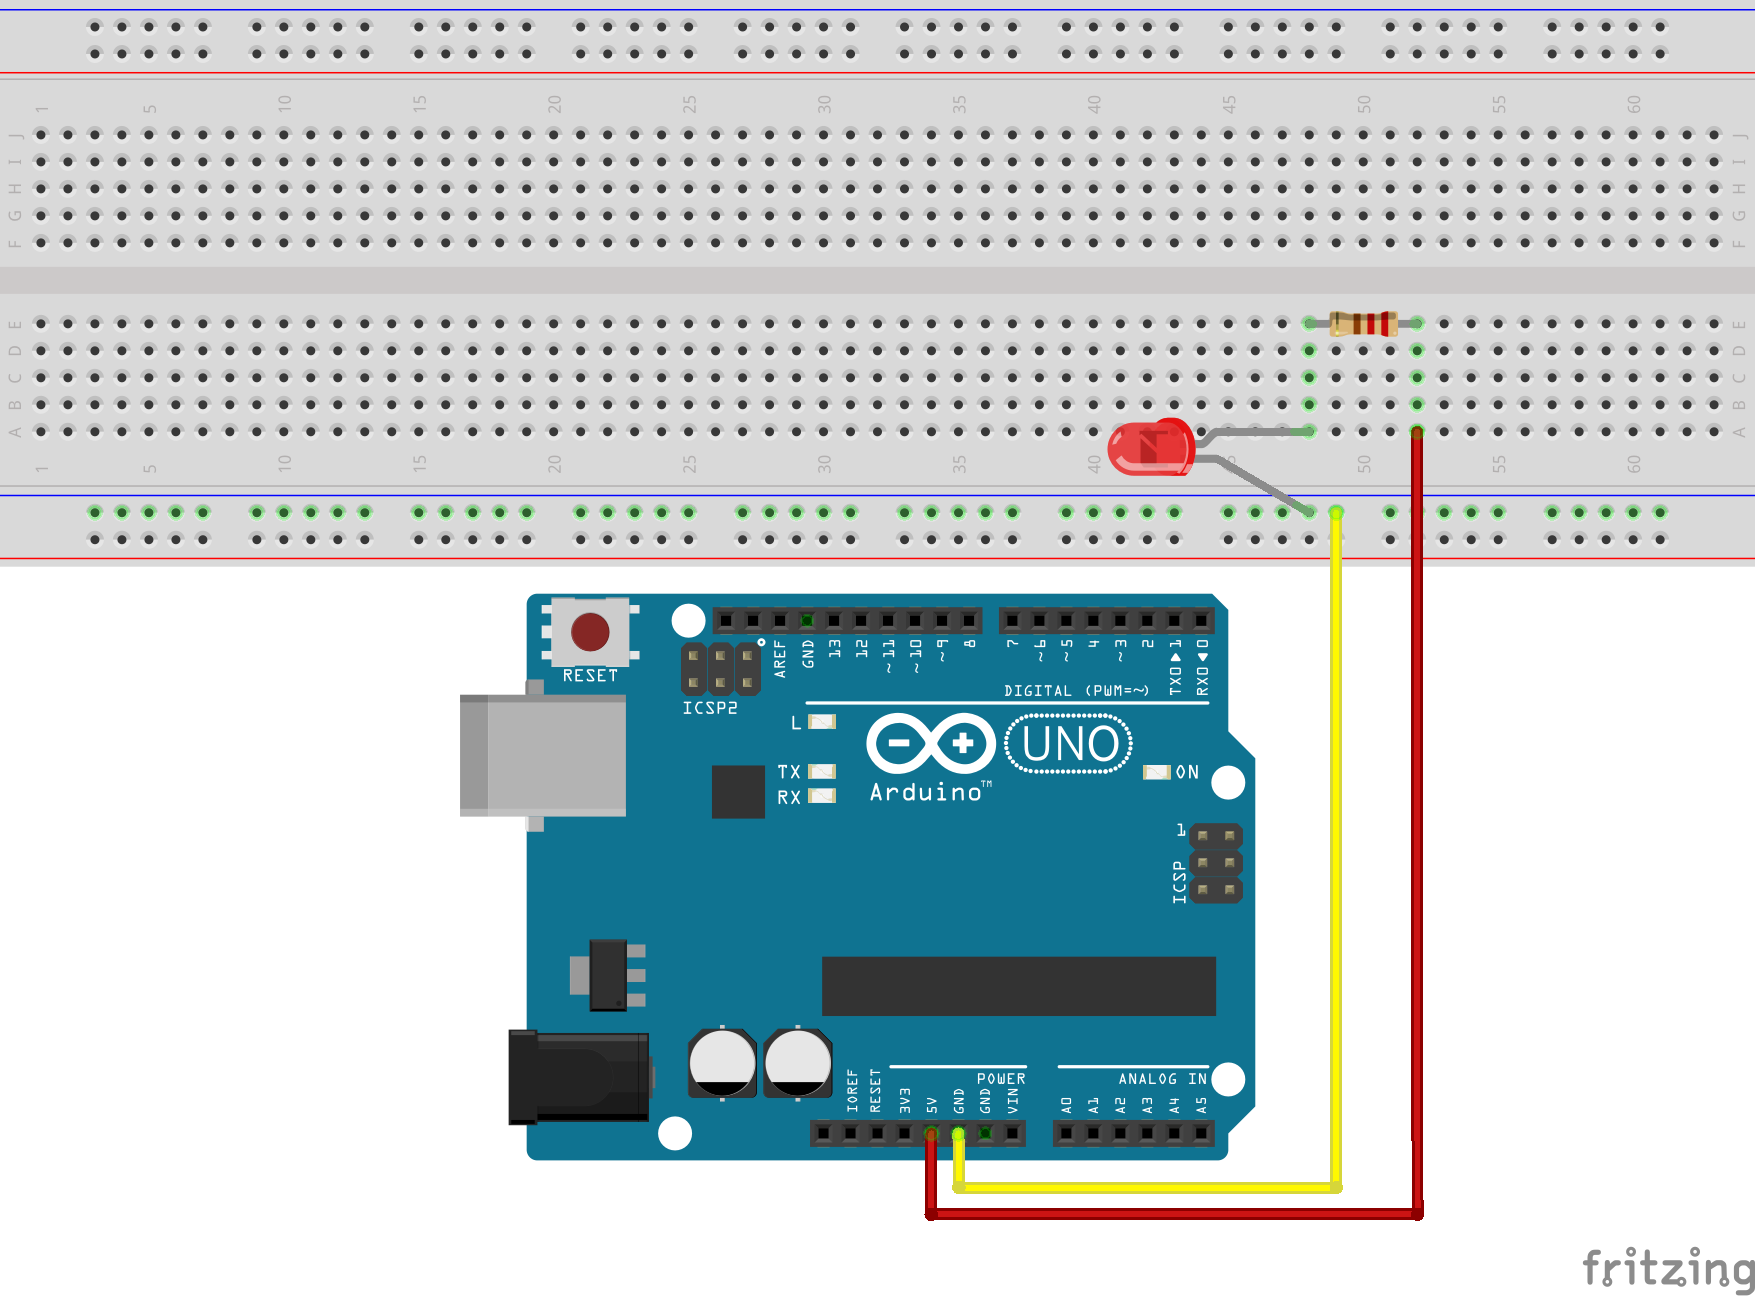
\includegraphics[width=12cm]{schematics/002-simple-arduino-circuit}
  \label{fig:breadboard-simple-arduino-circuit}
\end{figure}

Где номинал резистора $R_1$ должен быть не меньше 200 Ом.

Внимательно проверьте схему перед включением Arduino.  В первую очередь обратите
внимание на два провода, идущих от Arduino к макетной плате -- они не должны
замыкаться напрямую.  На схеме можно видеть, что провод от 5V идёт к ножке
резистора, а провод от GND (GROUND) идёт к ножке светодиода через общую линию,
отмеченную синим цветом, на макетной плате.

После включения питания, светодиод должен постоянно светиться.  Если он не
светится, необходимо отключить питание и ещё раз проверить собранную схему.
Одной из частых причин, почему светодиод не светится, является перепутанные плюс
и минус (анод и катод) на светодиоде; в этом случае, достаточно просто
перевернуть светодиод.

\experiment{0}{Попробуйте заменить резистор $R_1$ на резистор с большим
  сопротивлением (например, 500 Ом.)  Как изменилась яркость светодиода?}

Теперь попробуем выполнить последовательное подключение резисторов.  Для этого
возьмём два резистора, например, с номиналом от 200 до 300 Ом, и соберём
схему \ref{fig:electronics-arduino-circuit-00}.

\begin{figure}[ht]
  \centering
  \begin{circuitikz}
    \draw (4, 0) node [
      dipchip,
      num pins=2,
      external pins width=0.0,
      no topmark,
      hide numbers,
      xscale = 2.5,
      yscale = 2.5
    ](C1){Arduino};
    \node [above left, font=\small] at (C1.bpin 1) {5V};
    \node [above right, font=\small] at (C1.bpin 2) {GND};
    \draw
    (C1.bpin 1) to[short]
    (0, 0) to[short]
    (0, 4) to[resistor, l=$R_1$] (3, 4)
    (3, 4) to[resistor, l=$R_2$] (6, 4)
    (6, 4) to[full led, l=Светодиод] (8, 4)
    (8, 4) to[short]
    (8, 0) to[short]
    (C1.bpin 2);
  \end{circuitikz}
  \caption{Схема подключения светодиода к Arduino с последовательным
    подключением резисторов..}
  \label{fig:electronics-arduino-circuit-00}
\end{figure}

Если $R_1$ и $R_2$ равны допустим 200 Ом, то общее сопротивление цепи будет 400
Ом, как было показано в формуле \ref{equation:elemctronics-resistance-0}.

Итоговая схема показана на рис.
\ref{fig:breadboard-simple-arduino-circuit-resistor-in-series}.

\begin{figure}[ht]
  \centering
  \caption{Пример электрической цепи со светодиода и резисторами, подключенными
    последовательно.}
  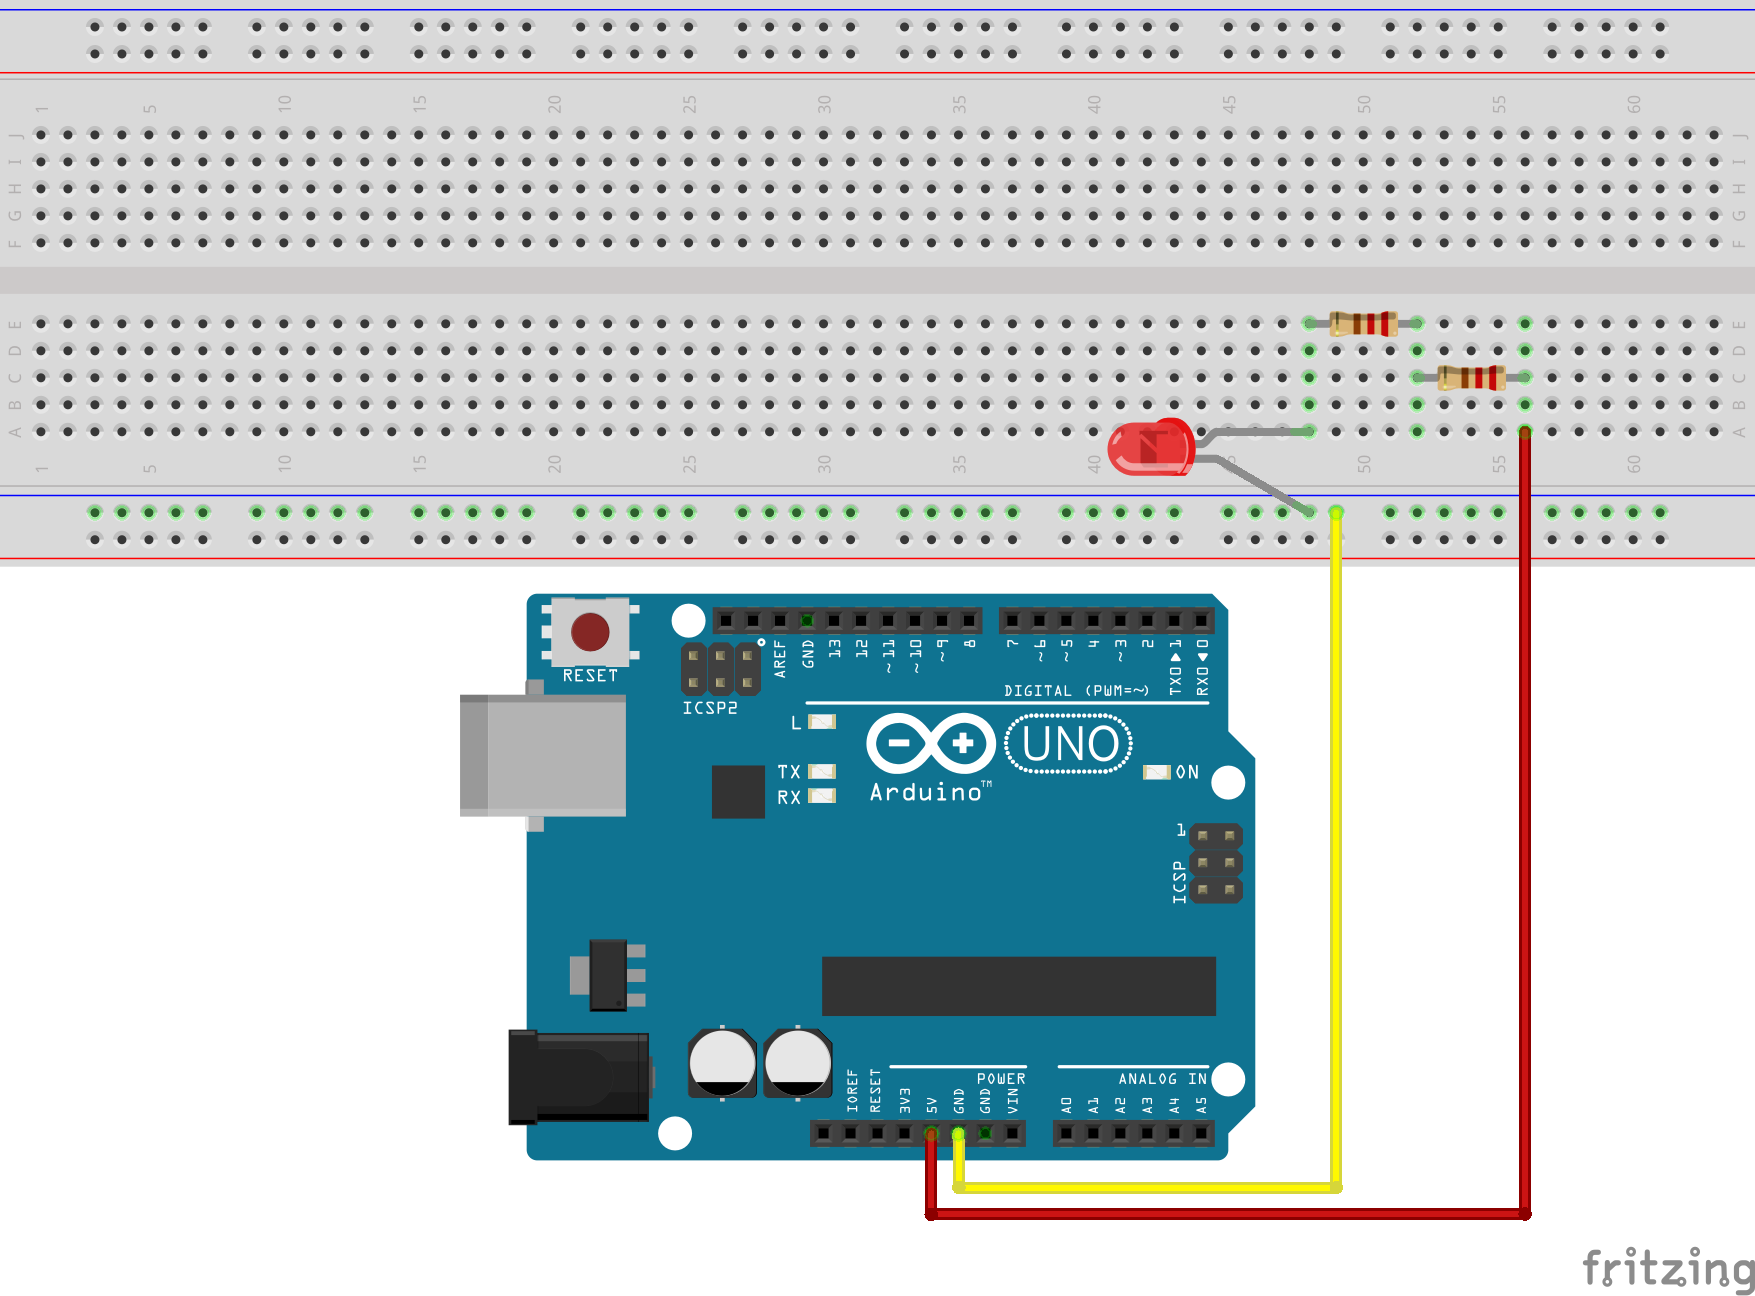
\includegraphics[width=12cm]{schematics/003-simple-arduino-circuit-resistor-in-series}
  \label{fig:breadboard-simple-arduino-circuit-resistor-in-series}
\end{figure}

\end{document}
